\subsection{Бонус: доступ из кода}

\begin{frame}[fragile]{Python}
\begin{minted}{python}
with sqlite3.Connection("literacy.sqlite3") as db:
  cursor = db.execute("SELECT * FROM Country LIMIT 3")
  print(cursor.description)
  print(list(cursor))
  print(list(cursor))  # Что-нибудь выведет?
\end{minted}
	\begin{itemize}
		\item Терминология очень похожа во всех языках и СУБД.
		\item Обычно в языке есть стандартный интерфейс общения с любыми СУБД.
			А \textit{драйвер} СУБД реализует этот интерфейс в языке.
		\item Сначала мы устанавливаем \textit{соединение} с СУБД.
		\item Результатом запроса является \textit{курсор} "--- это такой итератор по строчкам запроса.
		\item Что возвращают запросы, кроме \t{SELECT} "--- зависит от СУБД.
		\item
			Иногда считается, что не запрос возвращает курсор, а надо
			сначала создать курсор, а потом в нём выполнить запрос.
	\end{itemize}
\end{frame}

\begin{frame}[t,fragile]{SQL-инъекции}
	Пусть есть таблица с полями: владелец текста, его название, содержимое.
	Код для доступа к базе, выполняется на сервере:
\begin{minted}{python}
with sqlite3.Connection("sql-injection.sqlite3") as db:
  key = input('Text key: ')
  cursor = db.execute("""SELECT * FROM Text
                         WHERE owner='user' AND key='{}'"""
                         .format(key))
  print(list(cursor))
\end{minted}
	\only<1-2>{
	В чём проблема?
	\only<2>{
	\begin{center}
		\begin{tabular}{ll}
			Значение: & \t{key1} \\\hline
			Было:  & \t{SELECT ... WHERE owner='user' AND key='\{\}'} \\\hline
			Стало: & \t{SELECT ... WHERE owner='user' AND key='key1'} \\
		\end{tabular}
	\end{center}
	}
	}
	\only<3-4>{
	К коллайдеру!
	\only<4>{
	\begin{center}
		\begin{tabular}{ll}
			Значение: & \t{' OR ''='} \\\hline
			Было:  & \t{SELECT ... WHERE owner='user' AND key='\{\}'} \\\hline
			Стало: & \t{SELECT ... WHERE owner='user' AND key='' OR ''=''} \\
		\end{tabular}
	\end{center}
	Упс.
	}
	}
\end{frame}

\begin{frame}{Классический комикс}
	\begin{center}
		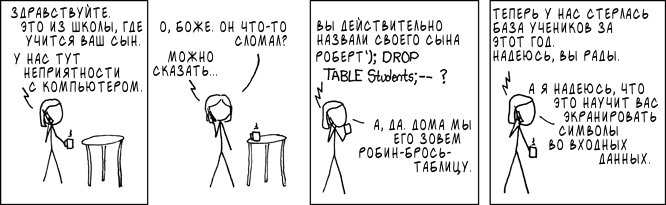
\includegraphics[scale=0.5]{xkcd-327.png}
	\end{center}
\end{frame}

\begin{frame}[fragile]{А как правильно?}
\begin{minted}{python}
with sqlite3.Connection("sql-injection.sqlite3") as db:
  key = input('Text key: ')
  cursor = db.execute("""SELECT * FROM Text
                         WHERE owner='user'
                           AND key=?""", [key])
  print(list(cursor))
\end{minted}
	Теперь драйвер базы данных знает, что \t{key} "--- это значение от пользователя,
	которое надо \textit{заэкранировать}:
	\begin{center}
		\begin{tabular}{ll}
			Значение: & \t{' OR ''='} \\\hline
			Было:  & \t{... WHERE owner='user' AND key=?} \\\hline
			Стало: & \t{... WHERE owner='user' AND key='\textbackslash' OR  \textbackslash'\textbackslash'=\textbackslash''} \\
		\end{tabular}
	\end{center}
	Независимо от того, какой код мы напишем, SQL-инъекции не случится.

	Мораль: никогда не собирайте SQL-запрос руками из переменных.
\end{frame}
